\PassOptionsToPackage{unicode=true}{hyperref} % options for packages loaded elsewhere
\PassOptionsToPackage{hyphens}{url}
%
\documentclass[]{article}
\usepackage{lmodern}
\usepackage{amssymb,amsmath}
\usepackage{ifxetex,ifluatex}
\usepackage{fixltx2e} % provides \textsubscript
\ifnum 0\ifxetex 1\fi\ifluatex 1\fi=0 % if pdftex
  \usepackage[T1]{fontenc}
  \usepackage[utf8]{inputenc}
  \usepackage{textcomp} % provides euro and other symbols
\else % if luatex or xelatex
  \usepackage{unicode-math}
  \defaultfontfeatures{Ligatures=TeX,Scale=MatchLowercase}
\fi
% use upquote if available, for straight quotes in verbatim environments
\IfFileExists{upquote.sty}{\usepackage{upquote}}{}
% use microtype if available
\IfFileExists{microtype.sty}{%
\usepackage[]{microtype}
\UseMicrotypeSet[protrusion]{basicmath} % disable protrusion for tt fonts
}{}
\IfFileExists{parskip.sty}{%
\usepackage{parskip}
}{% else
\setlength{\parindent}{0pt}
\setlength{\parskip}{6pt plus 2pt minus 1pt}
}
\usepackage{hyperref}
\hypersetup{
            pdftitle={Práctica en R del tema Clustering},
            pdfauthor={Laura Rodríguez Navas},
            pdfborder={0 0 0},
            breaklinks=true}
\urlstyle{same}  % don't use monospace font for urls
\usepackage[margin=1in]{geometry}
\usepackage{color}
\usepackage{fancyvrb}
\newcommand{\VerbBar}{|}
\newcommand{\VERB}{\Verb[commandchars=\\\{\}]}
\DefineVerbatimEnvironment{Highlighting}{Verbatim}{commandchars=\\\{\}}
% Add ',fontsize=\small' for more characters per line
\usepackage{framed}
\definecolor{shadecolor}{RGB}{248,248,248}
\newenvironment{Shaded}{\begin{snugshade}}{\end{snugshade}}
\newcommand{\AlertTok}[1]{\textcolor[rgb]{0.94,0.16,0.16}{#1}}
\newcommand{\AnnotationTok}[1]{\textcolor[rgb]{0.56,0.35,0.01}{\textbf{\textit{#1}}}}
\newcommand{\AttributeTok}[1]{\textcolor[rgb]{0.77,0.63,0.00}{#1}}
\newcommand{\BaseNTok}[1]{\textcolor[rgb]{0.00,0.00,0.81}{#1}}
\newcommand{\BuiltInTok}[1]{#1}
\newcommand{\CharTok}[1]{\textcolor[rgb]{0.31,0.60,0.02}{#1}}
\newcommand{\CommentTok}[1]{\textcolor[rgb]{0.56,0.35,0.01}{\textit{#1}}}
\newcommand{\CommentVarTok}[1]{\textcolor[rgb]{0.56,0.35,0.01}{\textbf{\textit{#1}}}}
\newcommand{\ConstantTok}[1]{\textcolor[rgb]{0.00,0.00,0.00}{#1}}
\newcommand{\ControlFlowTok}[1]{\textcolor[rgb]{0.13,0.29,0.53}{\textbf{#1}}}
\newcommand{\DataTypeTok}[1]{\textcolor[rgb]{0.13,0.29,0.53}{#1}}
\newcommand{\DecValTok}[1]{\textcolor[rgb]{0.00,0.00,0.81}{#1}}
\newcommand{\DocumentationTok}[1]{\textcolor[rgb]{0.56,0.35,0.01}{\textbf{\textit{#1}}}}
\newcommand{\ErrorTok}[1]{\textcolor[rgb]{0.64,0.00,0.00}{\textbf{#1}}}
\newcommand{\ExtensionTok}[1]{#1}
\newcommand{\FloatTok}[1]{\textcolor[rgb]{0.00,0.00,0.81}{#1}}
\newcommand{\FunctionTok}[1]{\textcolor[rgb]{0.00,0.00,0.00}{#1}}
\newcommand{\ImportTok}[1]{#1}
\newcommand{\InformationTok}[1]{\textcolor[rgb]{0.56,0.35,0.01}{\textbf{\textit{#1}}}}
\newcommand{\KeywordTok}[1]{\textcolor[rgb]{0.13,0.29,0.53}{\textbf{#1}}}
\newcommand{\NormalTok}[1]{#1}
\newcommand{\OperatorTok}[1]{\textcolor[rgb]{0.81,0.36,0.00}{\textbf{#1}}}
\newcommand{\OtherTok}[1]{\textcolor[rgb]{0.56,0.35,0.01}{#1}}
\newcommand{\PreprocessorTok}[1]{\textcolor[rgb]{0.56,0.35,0.01}{\textit{#1}}}
\newcommand{\RegionMarkerTok}[1]{#1}
\newcommand{\SpecialCharTok}[1]{\textcolor[rgb]{0.00,0.00,0.00}{#1}}
\newcommand{\SpecialStringTok}[1]{\textcolor[rgb]{0.31,0.60,0.02}{#1}}
\newcommand{\StringTok}[1]{\textcolor[rgb]{0.31,0.60,0.02}{#1}}
\newcommand{\VariableTok}[1]{\textcolor[rgb]{0.00,0.00,0.00}{#1}}
\newcommand{\VerbatimStringTok}[1]{\textcolor[rgb]{0.31,0.60,0.02}{#1}}
\newcommand{\WarningTok}[1]{\textcolor[rgb]{0.56,0.35,0.01}{\textbf{\textit{#1}}}}
\usepackage{graphicx,grffile}
\makeatletter
\def\maxwidth{\ifdim\Gin@nat@width>\linewidth\linewidth\else\Gin@nat@width\fi}
\def\maxheight{\ifdim\Gin@nat@height>\textheight\textheight\else\Gin@nat@height\fi}
\makeatother
% Scale images if necessary, so that they will not overflow the page
% margins by default, and it is still possible to overwrite the defaults
% using explicit options in \includegraphics[width, height, ...]{}
\setkeys{Gin}{width=\maxwidth,height=\maxheight,keepaspectratio}
\setlength{\emergencystretch}{3em}  % prevent overfull lines
\providecommand{\tightlist}{%
  \setlength{\itemsep}{0pt}\setlength{\parskip}{0pt}}
\setcounter{secnumdepth}{0}
% Redefines (sub)paragraphs to behave more like sections
\ifx\paragraph\undefined\else
\let\oldparagraph\paragraph
\renewcommand{\paragraph}[1]{\oldparagraph{#1}\mbox{}}
\fi
\ifx\subparagraph\undefined\else
\let\oldsubparagraph\subparagraph
\renewcommand{\subparagraph}[1]{\oldsubparagraph{#1}\mbox{}}
\fi

% set default figure placement to htbp
\makeatletter
\def\fps@figure{htbp}
\makeatother


\title{Práctica en R del tema Clustering}
\author{Laura Rodríguez Navas}
\date{10/07/2020}

\begin{document}
\maketitle

\hypertarget{parte-introductoria-de-la-pruxe1ctica}{%
\subsection{Parte introductoria de la
práctica}\label{parte-introductoria-de-la-pruxe1ctica}}

Para la correcta ejecución de esta práctica, el estudiante debe
verificar que los paquetes \textbf{mlbench} y \textbf{caret} están
correctamente instalados en la plataforma R. Para instalar estos
paquetes en R, solo debe ejecutar:

\begin{itemize}
\tightlist
\item
  \textbf{install.packages(``mlbench'')}
\item
  \textbf{install.packages(``caret'')}
\end{itemize}

Además, para esta práctica se ha decidido que se necesitan los
siguientes paquetes de R:

\begin{itemize}
\tightlist
\item
  \textbf{install.packages(``lattice'')}
\item
  \textbf{install.packages(``ggplot2'')}
\item
  \textbf{install.packages(``factoextra'')}
\item
  \textbf{install.packages(``ggdendro'')}
\item
  \textbf{install.packages(``cluster'')}
\end{itemize}

Luego de haber instalado los paquetes en R, pasamos a cargar en memoria
las librerías que usaremos.

\begin{Shaded}
\begin{Highlighting}[]
\KeywordTok{library}\NormalTok{(mlbench)}
\KeywordTok{library}\NormalTok{(lattice)}
\KeywordTok{library}\NormalTok{(ggplot2)}
\KeywordTok{library}\NormalTok{(caret)}
\KeywordTok{library}\NormalTok{(factoextra)}
\KeywordTok{library}\NormalTok{(ggdendro)}
\KeywordTok{library}\NormalTok{(cluster)}
\end{Highlighting}
\end{Shaded}

El paquete \textbf{mlbench} se utiliza para cargar los datasets con los
cuales trabajaremos en esta práctica. El paquete \textbf{caret} engloba
más de 200 modelos de clasificación así como funciones útiles para el
preprocesado de datos. A continuación cargamos el dataset BreastCancer
de la librería \textbf{mlbench}. El objetivo de este dataset es
describir si los pacientes tienen un cáncer benigno o maligno.

\begin{Shaded}
\begin{Highlighting}[]
\KeywordTok{data}\NormalTok{(BreastCancer)}
\end{Highlighting}
\end{Shaded}

El dataset ya se encuentra disponible en el entorno, ahora solo podrás
referenciarlo con la variable BreastCancer.

\hypertarget{ejercicios}{%
\subsection{Ejercicios}\label{ejercicios}}

A continuación debe resolver los siguientes ejercicios, escribiendo el
código en cada sección correspondiente después del comentario
\emph{\#INSERTAR CÓDIGO AQUÍ}.

\hypertarget{preprocesamiento-de-datos}{%
\subsubsection{Preprocesamiento de
datos}\label{preprocesamiento-de-datos}}

Describa brevemente el dataset BreastCancer. Puede apoyarse en las
funciones str(..) y summary (..). Como mínimo se espera que aporte la
siguiente información:

\begin{itemize}
\tightlist
\item
  Número de ejemplos (observaciones).
\item
  Número de variables.
\item
  Tipo de variables.
\item
  Distribuciones de datos por cada variable.
\item
  Número de valores perdidos.
\end{itemize}

\begin{Shaded}
\begin{Highlighting}[]
\CommentTok{#INSERTAR CÓDIGO AQUÍ}
\KeywordTok{str}\NormalTok{(BreastCancer, }\DataTypeTok{width =} \DecValTok{85}\NormalTok{, }\DataTypeTok{strict.width =} \StringTok{"cut"}\NormalTok{)}
\end{Highlighting}
\end{Shaded}

\begin{verbatim}
## 'data.frame':    699 obs. of  11 variables:
##  $ Id             : chr  "1000025" "1002945" "1015425" "1016277" ...
##  $ Cl.thickness   : Ord.factor w/ 10 levels "1"<"2"<"3"<"4"<..: 5 5 3 6 4 8 1 2 2 4..
##  $ Cell.size      : Ord.factor w/ 10 levels "1"<"2"<"3"<"4"<..: 1 4 1 8 1 10 1 1 1 ..
##  $ Cell.shape     : Ord.factor w/ 10 levels "1"<"2"<"3"<"4"<..: 1 4 1 8 1 10 1 2 1 ..
##  $ Marg.adhesion  : Ord.factor w/ 10 levels "1"<"2"<"3"<"4"<..: 1 5 1 1 3 8 1 1 1 1..
##  $ Epith.c.size   : Ord.factor w/ 10 levels "1"<"2"<"3"<"4"<..: 2 7 2 3 2 7 2 2 2 2..
##  $ Bare.nuclei    : Factor w/ 10 levels "1","2","3","4",..: 1 10 2 4 1 10 10 1 1 1 ..
##  $ Bl.cromatin    : Factor w/ 10 levels "1","2","3","4",..: 3 3 3 3 3 9 3 3 1 2 ...
##  $ Normal.nucleoli: Factor w/ 10 levels "1","2","3","4",..: 1 2 1 7 1 7 1 1 1 1 ...
##  $ Mitoses        : Factor w/ 9 levels "1","2","3","4",..: 1 1 1 1 1 1 1 1 5 1 ...
##  $ Class          : Factor w/ 2 levels "benign","malignant": 1 1 1 1 1 2 1 1 1 1 ...
\end{verbatim}

\begin{itemize}
\item
  Número de ejemplos (observaciones) = 699.
\item
  Número de variables = 11.
\item
  Tipo de variables. Consideramos el dataset BreastCancer definido sobre
  10 variables descriptoras (9 discretas, 5 de ellas ordenadas; y una
  variable de tipo carácter) y una variable clase binaria \{benign,
  malignant\}.
\item
  Distribuciones de datos por cada variable:
\end{itemize}

\begin{Shaded}
\begin{Highlighting}[]
\CommentTok{#INSERTAR CÓDIGO AQUÍ}
\KeywordTok{summary}\NormalTok{(BreastCancer)}
\end{Highlighting}
\end{Shaded}

\begin{verbatim}
##       Id             Cl.thickness   Cell.size     Cell.shape  Marg.adhesion
##  Length:699         1      :145   1      :384   1      :353   1      :407  
##  Class :character   5      :130   10     : 67   2      : 59   2      : 58  
##  Mode  :character   3      :108   3      : 52   10     : 58   3      : 58  
##                     4      : 80   2      : 45   3      : 56   10     : 55  
##                     10     : 69   4      : 40   4      : 44   4      : 33  
##                     2      : 50   5      : 30   5      : 34   8      : 25  
##                     (Other):117   (Other): 81   (Other): 95   (Other): 63  
##   Epith.c.size  Bare.nuclei   Bl.cromatin  Normal.nucleoli    Mitoses   
##  2      :386   1      :402   2      :166   1      :443     1      :579  
##  3      : 72   10     :132   3      :165   10     : 61     2      : 35  
##  4      : 48   2      : 30   1      :152   3      : 44     3      : 33  
##  1      : 47   5      : 30   7      : 73   2      : 36     10     : 14  
##  6      : 41   3      : 28   4      : 40   8      : 24     4      : 12  
##  5      : 39   (Other): 61   5      : 34   6      : 22     7      :  9  
##  (Other): 66   NA's   : 16   (Other): 69   (Other): 69     (Other): 17  
##        Class    
##  benign   :458  
##  malignant:241  
##                 
##                 
##                 
##                 
## 
\end{verbatim}

\newpage

\begin{itemize}
\tightlist
\item
  Número de valores perdidos.
\end{itemize}

\begin{Shaded}
\begin{Highlighting}[]
\CommentTok{#INSERTAR CÓDIGO AQUÍ}
\KeywordTok{sum}\NormalTok{(}\KeywordTok{is.na}\NormalTok{(BreastCancer))}
\end{Highlighting}
\end{Shaded}

\begin{verbatim}
## [1] 16
\end{verbatim}

\begin{itemize}
\tightlist
\item
  En caso de ser necesario, elimine los valores perdidos (R los
  representa como NA).
\end{itemize}

\begin{Shaded}
\begin{Highlighting}[]
\CommentTok{#INSERTAR CÓDIGO AQUÍ}
\NormalTok{BreastCancer <-}\StringTok{ }\KeywordTok{na.omit}\NormalTok{(BreastCancer) }
\KeywordTok{any}\NormalTok{(}\KeywordTok{is.na}\NormalTok{(BreastCancer))}
\end{Highlighting}
\end{Shaded}

\begin{verbatim}
## [1] FALSE
\end{verbatim}

Nota: en esta práctica, solo con la eliminación de registros es
suficiente. Sin embargo, tenga en cuenta que la eliminación de registros
que presentan valores perdidos no es una alternativa efectiva en la
mayoría de los casos.

\begin{itemize}
\tightlist
\item
  Ahora, transforma todas las variables descriptoras a tipo numérico.
  Esto es necesario porque muchos métodos de clustering trabajan
  solamente con variables numéricas.
\end{itemize}

\begin{Shaded}
\begin{Highlighting}[]
\CommentTok{#INSERTAR CÓDIGO AQUÍ}
\ControlFlowTok{for}\NormalTok{ (i }\ControlFlowTok{in} \DecValTok{1}\OperatorTok{:}\NormalTok{(}\KeywordTok{ncol}\NormalTok{(BreastCancer) }\OperatorTok{-}\StringTok{ }\DecValTok{1}\NormalTok{))}
\NormalTok{  BreastCancer[, i] <-}\StringTok{ }\KeywordTok{as.numeric}\NormalTok{(}\KeywordTok{as.character}\NormalTok{(BreastCancer[, i]))}

\KeywordTok{str}\NormalTok{(BreastCancer, }\DataTypeTok{width =} \DecValTok{85}\NormalTok{, }\DataTypeTok{strict.width =} \StringTok{"cut"}\NormalTok{)}
\end{Highlighting}
\end{Shaded}

\begin{verbatim}
## 'data.frame':    683 obs. of  11 variables:
##  $ Id             : num  1000025 1002945 1015425 1016277 1017023 ...
##  $ Cl.thickness   : num  5 5 3 6 4 8 1 2 2 4 ...
##  $ Cell.size      : num  1 4 1 8 1 10 1 1 1 2 ...
##  $ Cell.shape     : num  1 4 1 8 1 10 1 2 1 1 ...
##  $ Marg.adhesion  : num  1 5 1 1 3 8 1 1 1 1 ...
##  $ Epith.c.size   : num  2 7 2 3 2 7 2 2 2 2 ...
##  $ Bare.nuclei    : num  1 10 2 4 1 10 10 1 1 1 ...
##  $ Bl.cromatin    : num  3 3 3 3 3 9 3 3 1 2 ...
##  $ Normal.nucleoli: num  1 2 1 7 1 7 1 1 1 1 ...
##  $ Mitoses        : num  1 1 1 1 1 1 1 1 5 1 ...
##  $ Class          : Factor w/ 2 levels "benign","malignant": 1 1 1 1 1 2 1 1 1 1 ...
##  - attr(*, "na.action")= 'omit' Named int [1:16] 24 41 140 146 159 165 236 250 276 ..
##   ..- attr(*, "names")= chr [1:16] "24" "41" "140" "146" ...
\end{verbatim}

\begin{itemize}
\tightlist
\item
  La variable ``ID'' representa un identificador que es único para cada
  paciente y no aporta ninguna información para el aprendizaje
  automático, por lo que podemos eliminarlo con seguridad.
\end{itemize}

\begin{Shaded}
\begin{Highlighting}[]
\CommentTok{#INSERTAR CÓDIGO AQUÍ}
\NormalTok{BreastCancer}\OperatorTok{$}\NormalTok{Id <-}\StringTok{ }\OtherTok{NULL}
\KeywordTok{head}\NormalTok{(BreastCancer, }\DecValTok{3}\NormalTok{)}
\end{Highlighting}
\end{Shaded}

\begin{verbatim}
##   Cl.thickness Cell.size Cell.shape Marg.adhesion Epith.c.size Bare.nuclei
## 1            5         1          1             1            2           1
## 2            5         4          4             5            7          10
## 3            3         1          1             1            2           2
##   Bl.cromatin Normal.nucleoli Mitoses  Class
## 1           3               1       1 benign
## 2           3               2       1 benign
## 3           3               1       1 benign
\end{verbatim}

\begin{itemize}
\tightlist
\item
  Debido a que los algoritmos de clustering se basan en el cómputo de
  valores de distancias entre los ejemplos, es ventajoso tener todas las
  variables en la misma escala para el cálculo de las distancias entre
  ejemplos. Convierta todos los atributos descriptores a una misma
  escala.
\end{itemize}

Nota: se recomienda utilizar la función preProcess(.., method =
``scale'') de la librería caret.

\begin{Shaded}
\begin{Highlighting}[]
\CommentTok{# INSERTAR CÓDIGO AQUÍ}
\NormalTok{BreastCancer.scale <-}\StringTok{ }\KeywordTok{preProcess}\NormalTok{(BreastCancer[, }\DecValTok{1}\OperatorTok{:}\DecValTok{9}\NormalTok{], }\DataTypeTok{method=}\KeywordTok{c}\NormalTok{(}\StringTok{"scale"}\NormalTok{))}
\NormalTok{BreastCancer.features <-}\StringTok{ }\KeywordTok{predict}\NormalTok{(BreastCancer.scale, BreastCancer[, }\DecValTok{1}\OperatorTok{:}\DecValTok{9}\NormalTok{])}
\KeywordTok{str}\NormalTok{(BreastCancer.features, }\DataTypeTok{width =} \DecValTok{85}\NormalTok{, }\DataTypeTok{strict.width =} \StringTok{"cut"}\NormalTok{)}
\end{Highlighting}
\end{Shaded}

\begin{verbatim}
## 'data.frame':    683 obs. of  9 variables:
##  $ Cl.thickness   : num  1.77 1.77 1.06 2.13 1.42 ...
##  $ Cell.size      : num  0.326 1.305 0.326 2.61 0.326 ...
##  $ Cell.shape     : num  0.335 1.338 0.335 2.677 0.335 ...
##  $ Marg.adhesion  : num  0.349 1.745 0.349 0.349 1.047 ...
##  $ Epith.c.size   : num  0.9 3.15 0.9 1.35 0.9 ...
##  $ Bare.nuclei    : num  0.274 2.744 0.549 1.098 0.274 ...
##  $ Bl.cromatin    : num  1.22 1.22 1.22 1.22 1.22 ...
##  $ Normal.nucleoli: num  0.328 0.655 0.328 2.293 0.328 ...
##  $ Mitoses        : num  0.577 0.577 0.577 0.577 0.577 ...
\end{verbatim}

\hypertarget{clustering-con-kmeans}{%
\subsubsection{Clustering con kMeans}\label{clustering-con-kmeans}}

Una vez que los datos han sido preprocesados, la librería ggplot2, la
cual es automaticamente importada por la librería caret, nos permite
visualizar los datos para comprobar cómo las diferentes variables
afectan al tipo de cáncer.

\begin{Shaded}
\begin{Highlighting}[]
\CommentTok{# En este caso solo estamos mostrando el gráfico para las variables Cl.thickness y Cell.size.}
\KeywordTok{ggplot}\NormalTok{(BreastCancer, }\KeywordTok{aes}\NormalTok{(Cl.thickness, Cell.size, }\DataTypeTok{color =}\NormalTok{ Class)) }\OperatorTok{+}\StringTok{ }\KeywordTok{geom_point}\NormalTok{()}
\end{Highlighting}
\end{Shaded}

\begin{center}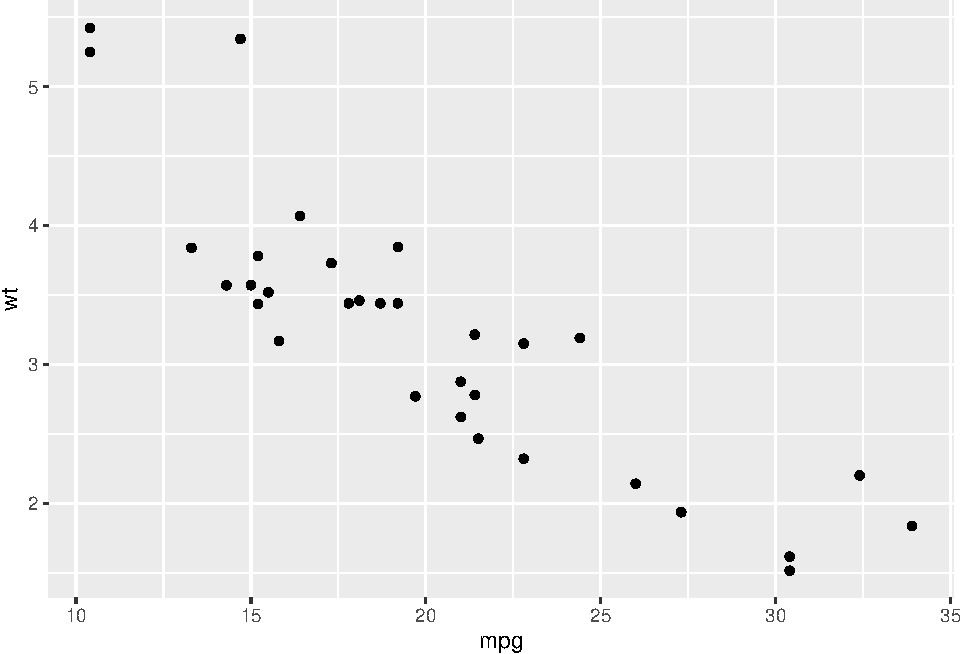
\includegraphics[width=0.7\linewidth]{Práctica-R-Clustering_files/figure-latex/unnamed-chunk-10-1} \end{center}

Se puede apreciar que considerando estos pares de variables se observan
dos grupos claramente definidos.

\begin{itemize}
\tightlist
\item
  Pasemos ahora a ejecutar algoritmos de clustering sobre nuestros
  datos. Mediante un agrupamiento usando kmeans(..), encuentre el par de
  variables descriptoras a partir del cual se logra un mejor
  agrupamiento. Utilice 20 asignaciones aleatorias para inicializar los
  centroides y además fije el número de cluster igual al número de
  clases existentes en el dataset.
\end{itemize}

Nota: recuerde que la variable Class no se debe tener en cuenta a la
hora de realizar el clustering, ya que estamos haciendo un aprendizaje
no supervisado. El atributo Class es útil para usar una métrica de
evaluación externa y así comprobar la calidad del agrupamiento.

\begin{Shaded}
\begin{Highlighting}[]
\CommentTok{#INSERTAR CÓDIGO AQUÍ}
\KeywordTok{set.seed}\NormalTok{(}\DecValTok{101}\NormalTok{)}
\NormalTok{km_clusters <-}\StringTok{ }\KeywordTok{kmeans}\NormalTok{(BreastCancer.features, }\DataTypeTok{centers =} \DecValTok{2}\NormalTok{, }\DataTypeTok{nstart =} \DecValTok{20}\NormalTok{)}
\NormalTok{km_clusters}
\end{Highlighting}
\end{Shaded}

\begin{verbatim}
## K-means clustering with 2 clusters of sizes 453, 230
## 
## Cluster means:
##   Cl.thickness Cell.size Cell.shape Marg.adhesion Epith.c.size Bare.nuclei
## 1     1.077629 0.4191542  0.4712566     0.4700817    0.9423492   0.3840871
## 2     2.554044 2.2270031  2.2665986     2.0080464    2.4642601   2.1322365
##   Bl.cromatin Normal.nucleoli  Mitoses
## 1   0.8578798       0.4092973 0.617912
## 2   2.4865546       1.9854346 1.530682
## 
## Clustering vector:
##   1   2   3   4   5   6   7   8   9  10  11  12  13  14  15  16  17  18  19  20 
##   1   2   1   2   1   2   1   1   1   1   1   1   1   1   2   2   1   1   2   1 
##  21  22  23  25  26  27  28  29  30  31  32  33  34  35  36  37  38  39  40  42 
##   2   2   1   1   1   1   1   1   1   1   1   2   1   1   1   2   1   2   2   2 
##  43  44  45  46  47  48  49  50  51  52  53  54  55  56  57  58  59  60  61  62 
##   2   2   2   1   2   1   1   2   2   1   2   2   2   2   2   1   1   1   2   1 
##  63  64  65  66  67  68  69  70  71  72  73  74  75  76  77  78  79  80  81  82 
##   2   1   1   2   1   2   2   1   1   2   1   2   2   1   1   1   1   1   1   1 
##  83  84  85  86  87  88  89  90  91  92  93  94  95  96  97  98  99 100 101 102 
##   1   1   2   2   2   2   1   1   1   1   1   1   1   1   1   1   2   2   2   1 
## 103 104 105 106 107 108 109 110 111 112 113 114 115 116 117 118 119 120 121 122 
##   1   1   2   2   2   2   1   2   1   2   2   2   1   1   1   2   1   1   1   1 
## 123 124 125 126 127 128 129 130 131 132 133 134 135 136 137 138 139 141 142 143 
##   2   2   2   1   2   1   2   1   1   1   2   1   1   1   1   1   1   1   1   2 
## 144 145 147 148 149 150 151 152 153 154 155 156 157 158 160 161 162 163 164 166 
##   1   1   1   1   1   2   1   2   2   1   1   2   1   1   2   2   1   1   1   1 
## 167 168 169 170 171 172 173 174 175 176 177 178 179 180 181 182 183 184 185 186 
##   2   2   1   1   1   1   1   2   2   2   1   2   1   1   1   1   1   2   2   1 
## 187 188 189 190 191 192 193 194 195 196 197 198 199 200 201 202 203 204 205 206 
##   2   2   2   1   2   2   1   1   1   1   2   1   1   1   2   2   1   1   1   2 
## 207 208 209 210 211 212 213 214 215 216 217 218 219 220 221 222 223 224 225 226 
##   2   1   1   1   2   2   1   2   2   2   1   1   2   1   1   2   1   2   2   1 
## 227 228 229 230 231 232 233 234 235 237 238 239 240 241 242 243 244 245 246 247 
##   2   2   1   2   2   2   1   2   1   2   2   2   2   1   1   1   1   1   1   2 
## 248 249 251 252 253 254 255 256 257 258 259 260 261 262 263 264 265 266 267 268 
##   1   1   1   2   2   2   2   2   1   1   1   2   2   2   2   2   2   1   2   2 
## 269 270 271 272 273 274 275 277 278 279 280 281 282 283 284 285 286 287 288 289 
##   2   1   2   1   2   1   1   1   1   1   2   1   1   2   2   2   2   2   1   2 
## 290 291 292 294 296 297 299 300 301 302 303 304 305 306 307 308 309 310 311 312 
##   2   1   1   2   2   2   1   2   2   1   2   1   2   2   1   1   2   1   1   1 
## 313 314 315 317 318 319 320 321 323 324 325 326 327 328 329 330 331 332 333 334 
##   2   1   1   2   2   1   2   2   1   2   1   1   1   1   2   2   2   1   1   2 
## 335 336 337 338 339 340 341 342 343 344 345 346 347 348 349 350 351 352 353 354 
##   2   1   2   1   1   2   2   1   1   1   2   1   1   1   1   2   1   1   2   2 
## 355 356 357 358 359 360 361 362 363 364 365 366 367 368 369 370 371 372 373 374 
##   1   1   1   2   2   2   2   2   1   1   1   1   2   2   1   1   1   1   1   1 
## 375 376 377 378 379 380 381 382 383 384 385 386 387 388 389 390 391 392 393 394 
##   1   1   1   1   1   1   1   2   1   1   1   1   2   1   1   1   1   2   1   1 
## 395 396 397 398 399 400 401 402 403 404 405 406 407 408 409 410 411 413 414 415 
##   1   1   1   1   1   1   2   1   1   1   1   1   1   1   1   1   1   2   1   2 
## 416 417 418 419 420 421 422 423 424 425 426 427 428 429 430 431 432 433 434 435 
##   1   2   1   1   1   1   2   1   1   1   2   1   2   1   1   1   1   1   1   2 
## 436 437 438 439 440 441 442 443 444 445 446 447 448 449 450 451 452 453 454 455 
##   2   2   1   1   1   2   1   1   1   1   1   1   1   1   2   1   1   1   2   1 
## 456 457 458 459 460 461 462 463 464 465 466 467 468 469 470 471 472 473 474 475 
##   1   2   2   1   1   1   1   1   1   1   2   2   2   1   1   1   1   1   1   1 
## 476 477 478 479 480 481 482 483 484 485 486 487 488 489 490 491 492 493 494 495 
##   1   1   1   1   2   1   1   2   2   1   1   1   2   2   1   1   2   1   2   1 
## 496 497 498 499 500 501 502 503 504 505 506 507 508 509 510 511 512 513 514 515 
##   1   1   1   1   1   1   1   1   1   1   1   2   1   1   1   1   1   1   1   2 
## 516 517 518 519 520 521 522 523 524 525 526 527 528 529 530 531 532 533 534 535 
##   2   1   1   1   2   1   1   2   2   1   1   1   1   1   1   2   1   1   1   1 
## 536 537 538 539 540 541 542 543 544 545 546 547 548 549 550 551 552 553 554 555 
##   1   1   1   1   1   1   1   1   1   1   1   2   1   1   2   1   1   1   1   1 
## 556 557 558 559 560 561 562 563 564 565 566 567 568 569 570 571 572 573 574 575 
##   1   1   1   1   1   1   1   1   1   1   2   1   1   2   2   2   2   1   1   2 
## 576 577 578 579 580 581 582 583 584 585 586 587 588 589 590 591 592 593 594 595 
##   1   1   1   1   1   1   2   2   1   1   1   2   1   2   1   2   2   2   1   2 
## 596 597 598 599 600 601 602 603 604 605 606 607 608 609 610 611 612 613 614 615 
##   1   1   1   1   1   1   1   1   2   2   2   1   1   2   1   2   2   2   1   1 
## 616 617 619 620 621 622 623 624 625 626 627 628 629 630 631 632 633 634 635 636 
##   1   1   1   1   1   1   1   1   1   1   2   1   1   1   1   1   1   2   1   1 
## 637 638 639 640 641 642 643 644 645 646 647 648 649 650 651 652 653 654 655 656 
##   2   1   1   1   1   1   1   1   1   1   1   1   2   1   1   1   1   1   1   1 
## 657 658 659 660 661 662 663 664 665 666 667 668 669 670 671 672 673 674 675 676 
##   1   2   2   1   1   1   1   1   1   1   1   1   2   2   2   1   1   1   1   1 
## 677 678 679 680 681 682 683 684 685 686 687 688 689 690 691 692 693 694 695 696 
##   1   1   1   1   2   2   1   1   1   1   1   1   1   1   1   2   1   1   1   1 
## 697 698 699 
##   2   2   2 
## 
## Within cluster sum of squares by cluster:
## [1]  573.4613 2150.6939
##  (between_SS / total_SS =  55.6 %)
## 
## Available components:
## 
## [1] "cluster"      "centers"      "totss"        "withinss"     "tot.withinss"
## [6] "betweenss"    "size"         "iter"         "ifault"
\end{verbatim}

\begin{itemize}
\tightlist
\item
  A partir de los resultados obtenidos, ¿Por qué se puede considerar un
  buen agrupamiento? Justifica de forma clara y concisa la elección del
  par de atributos. Puedes ayudarte con la funciones table(..) y
  ggplot(..) para justificar tu respuesta.
\end{itemize}

RESPUESTA:

\begin{Shaded}
\begin{Highlighting}[]
\CommentTok{#INSERTAR CÓDIGO AQUÍ}
\KeywordTok{fviz_cluster}\NormalTok{(km_clusters, }\DataTypeTok{data =}\NormalTok{ BreastCancer.features,}
             \DataTypeTok{ggtheme =} \KeywordTok{theme_minimal}\NormalTok{(),}
             \DataTypeTok{main =} \StringTok{"Partitioning Clustering Plot"}\NormalTok{)}
\end{Highlighting}
\end{Shaded}

\begin{center}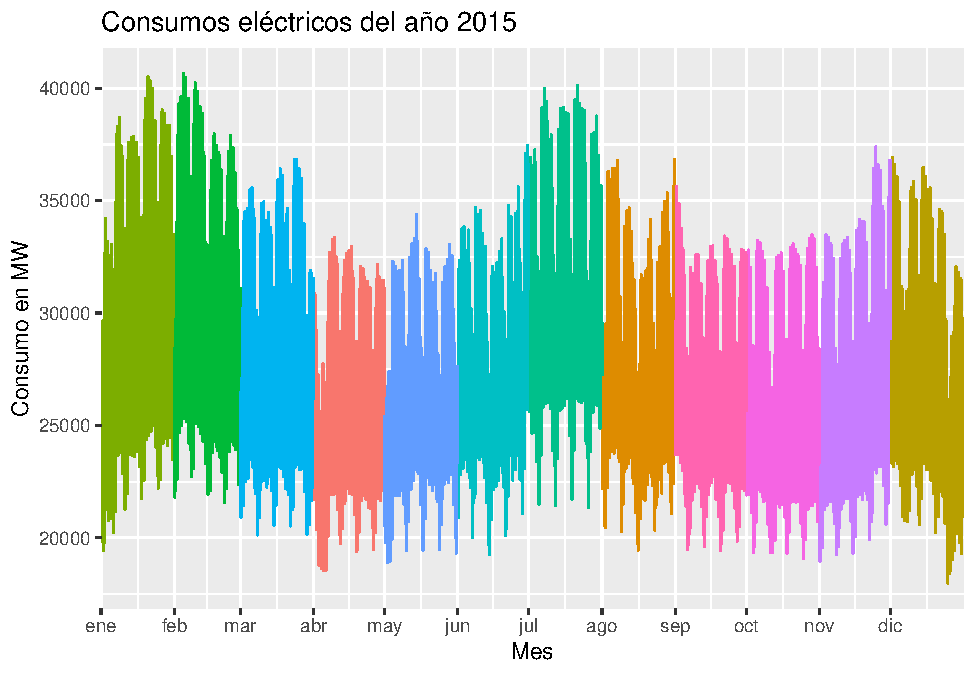
\includegraphics[width=0.7\linewidth]{Práctica-R-Clustering_files/figure-latex/unnamed-chunk-12-1} \end{center}

La propia función (\emph{fviz\_cluster}) determina las dos dimensiones,
es decir, el par de variables más representativo en el dataset.

Si observamos la anterior figura, el agrupamiento no ha sido del todo
bueno. Los clusters no acaban de verse bien diferenciados, y se puede
observar un poco de \emph{overlapping} entre ellos.

Para la validación de los clusters se utiliza el coeficiente de
Silhouette: un valor de Si cercano a 1 indica que el cluster estará bien
agrupado. Un valor de Si cercano a -1 indicará que el cluster estará mal
agrupado.

A continuación vemos la representación del coeficiente de Silhouette:

\begin{Shaded}
\begin{Highlighting}[]
\CommentTok{#INSERTAR CÓDIGO AQUÍ}
\NormalTok{sil <-}\StringTok{ }\KeywordTok{silhouette}\NormalTok{(km_clusters}\OperatorTok{$}\NormalTok{cluster, }\KeywordTok{dist}\NormalTok{(BreastCancer.features))}
\KeywordTok{fviz_silhouette}\NormalTok{(sil)}
\end{Highlighting}
\end{Shaded}

\begin{verbatim}
##   cluster size ave.sil.width
## 1       1  453          0.75
## 2       2  230          0.23
\end{verbatim}

\begin{center}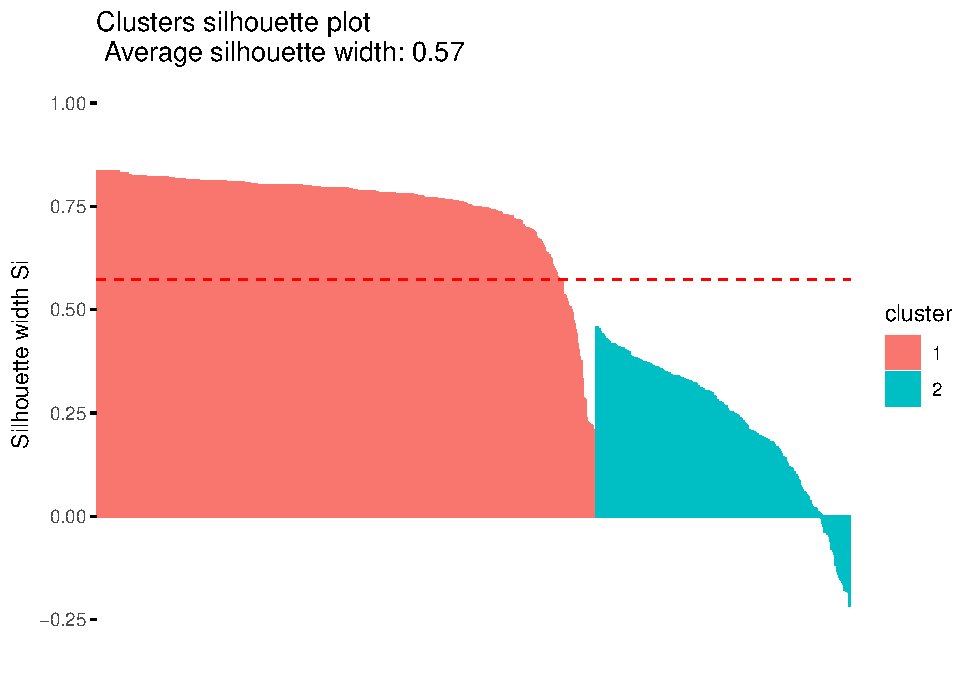
\includegraphics[width=0.7\linewidth]{Práctica-R-Clustering_files/figure-latex/unnamed-chunk-13-1} \end{center}

\begin{itemize}
\item
  Mediante la función preprocess(..) de la librería caret, analice si se
  obtienen mejores resultados de agrupamiento con el par de atributos
  seleccionados anteriormente, pero en este caso haciendo inicialmente
  las siguientes combinaciones de transformaciones a los datos:

  \begin{itemize}
  \tightlist
  \item
    c(``center'', ``scale'')
  \item
    c(``center'', ``scale'', ``YeoJohnson'')
  \item
    c(``range'')
  \item
    c(``range'', ``YeoJohnson'')
  \end{itemize}
\end{itemize}

Ayúdate de los resultados obtenidos con table y ggplot.

\begin{itemize}
\tightlist
\item
  c(``center'', ``scale'')
\end{itemize}

\begin{Shaded}
\begin{Highlighting}[]
\CommentTok{#INSERTAR CÓDIGO AQUÍ}
\NormalTok{BreastCancer.scale <-}\StringTok{ }\KeywordTok{preProcess}\NormalTok{(BreastCancer[, }\DecValTok{1}\OperatorTok{:}\DecValTok{9}\NormalTok{], }\DataTypeTok{method=}\KeywordTok{c}\NormalTok{(}\StringTok{"center"}\NormalTok{, }\StringTok{"scale"}\NormalTok{))}
\NormalTok{BreastCancer.features <-}\StringTok{ }\KeywordTok{predict}\NormalTok{(BreastCancer.scale, BreastCancer[, }\DecValTok{1}\OperatorTok{:}\DecValTok{9}\NormalTok{])}
\KeywordTok{set.seed}\NormalTok{(}\DecValTok{101}\NormalTok{)}
\NormalTok{km_clusters <-}\StringTok{ }\KeywordTok{kmeans}\NormalTok{(BreastCancer.features, }\DataTypeTok{centers =} \DecValTok{2}\NormalTok{, }\DataTypeTok{nstart =} \DecValTok{20}\NormalTok{)}
\KeywordTok{fviz_cluster}\NormalTok{(km_clusters, }\DataTypeTok{data =}\NormalTok{ BreastCancer.features,}
             \DataTypeTok{ggtheme =} \KeywordTok{theme_minimal}\NormalTok{(),}
             \DataTypeTok{main =} \StringTok{"Partitioning Clustering Plot"}\NormalTok{)}
\end{Highlighting}
\end{Shaded}

\begin{center}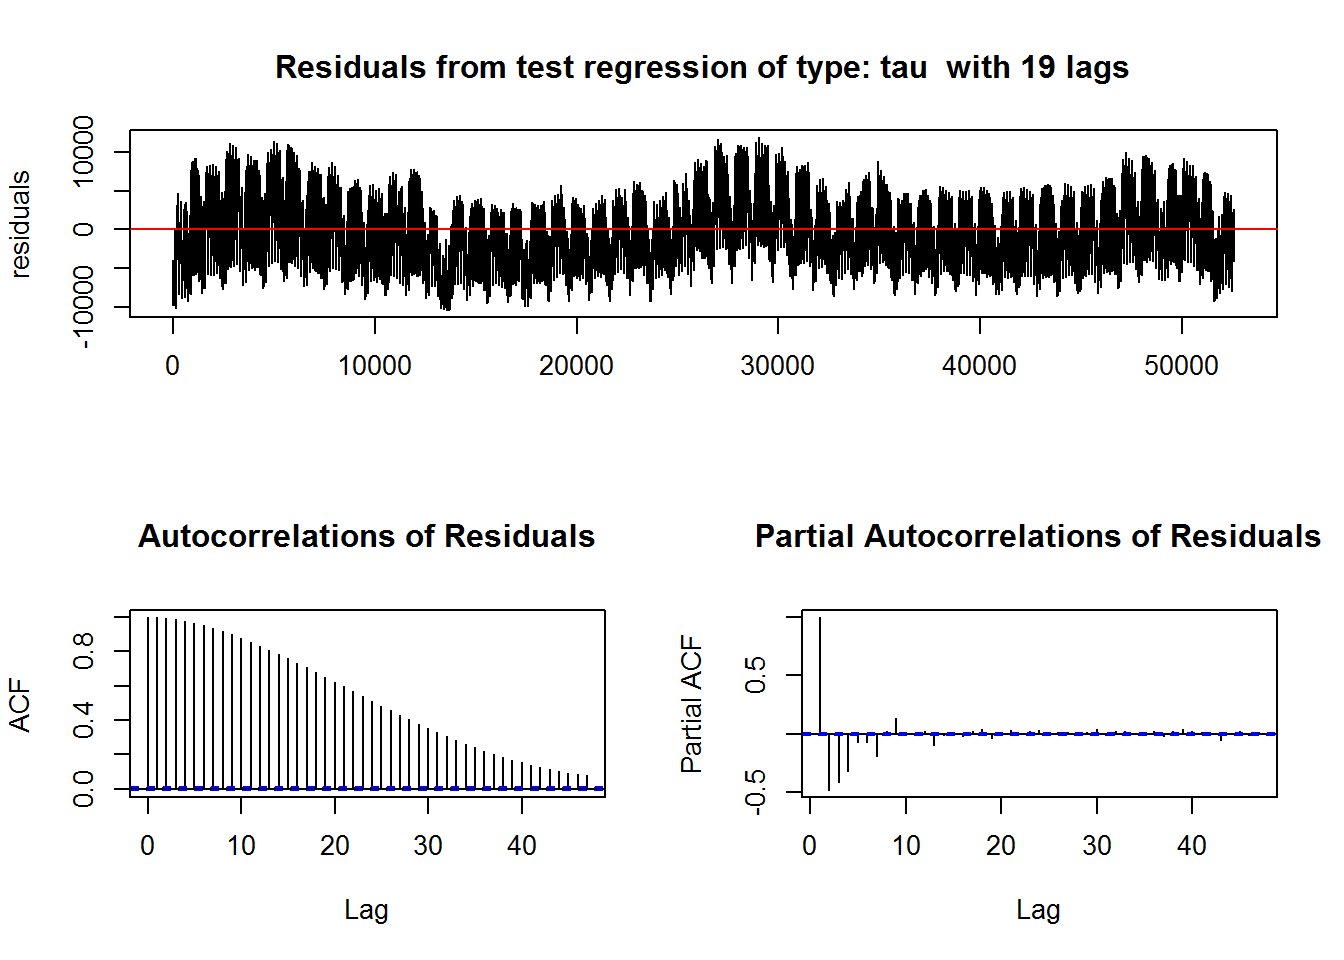
\includegraphics[width=0.7\linewidth]{Práctica-R-Clustering_files/figure-latex/unnamed-chunk-14-1} \end{center}

\begin{Shaded}
\begin{Highlighting}[]
\NormalTok{sil <-}\StringTok{ }\KeywordTok{silhouette}\NormalTok{(km_clusters}\OperatorTok{$}\NormalTok{cluster, }\KeywordTok{dist}\NormalTok{(BreastCancer.features))}
\KeywordTok{fviz_silhouette}\NormalTok{(sil)}
\end{Highlighting}
\end{Shaded}

\begin{verbatim}
##   cluster size ave.sil.width
## 1       1  453          0.75
## 2       2  230          0.23
\end{verbatim}

\begin{center}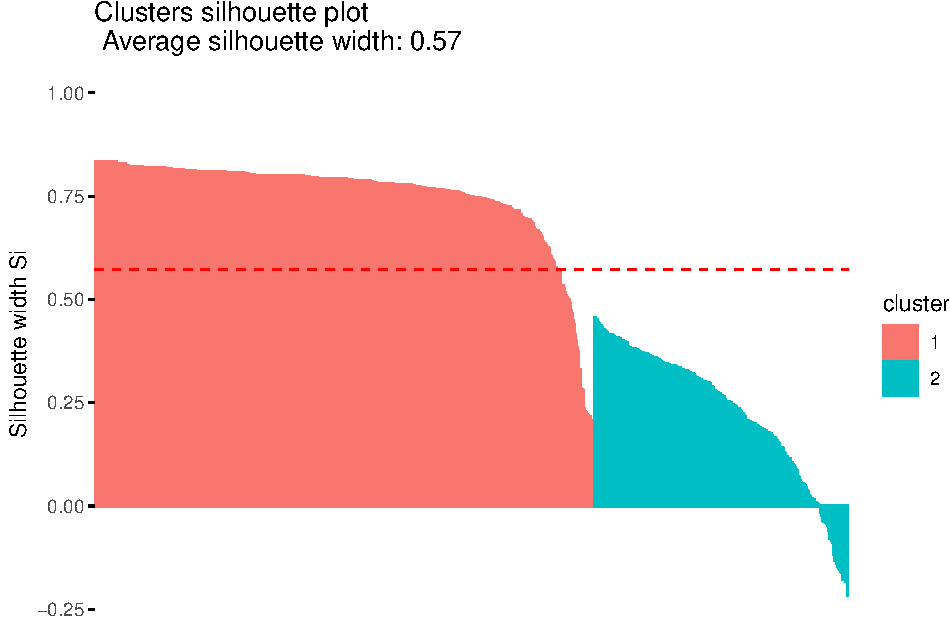
\includegraphics[width=0.7\linewidth]{Práctica-R-Clustering_files/figure-latex/unnamed-chunk-14-2} \end{center}

El resultado de agrupamiento no presenta mejoras.

\begin{itemize}
\tightlist
\item
  c(``center'', ``scale'', ``YeoJohnson'')
\end{itemize}

\begin{Shaded}
\begin{Highlighting}[]
\CommentTok{#INSERTAR CÓDIGO AQUÍ}
\NormalTok{BreastCancer.scale <-}\StringTok{ }\KeywordTok{preProcess}\NormalTok{(BreastCancer[, }\DecValTok{1}\OperatorTok{:}\DecValTok{9}\NormalTok{], }\DataTypeTok{method=}\KeywordTok{c}\NormalTok{(}\StringTok{"center"}\NormalTok{, }\StringTok{"scale"}\NormalTok{, }\StringTok{"YeoJohnson"}\NormalTok{))}
\NormalTok{BreastCancer.features <-}\StringTok{ }\KeywordTok{predict}\NormalTok{(BreastCancer.scale, BreastCancer[, }\DecValTok{1}\OperatorTok{:}\DecValTok{9}\NormalTok{])}
\KeywordTok{set.seed}\NormalTok{(}\DecValTok{101}\NormalTok{)}
\NormalTok{km_clusters <-}\StringTok{ }\KeywordTok{kmeans}\NormalTok{(BreastCancer.features, }\DataTypeTok{centers =} \DecValTok{2}\NormalTok{, }\DataTypeTok{nstart =} \DecValTok{20}\NormalTok{)}
\KeywordTok{fviz_cluster}\NormalTok{(km_clusters, }\DataTypeTok{data =}\NormalTok{ BreastCancer.features,}
             \DataTypeTok{ggtheme =} \KeywordTok{theme_minimal}\NormalTok{(),}
             \DataTypeTok{main =} \StringTok{"Partitioning Clustering Plot"}\NormalTok{)}
\end{Highlighting}
\end{Shaded}

\begin{center}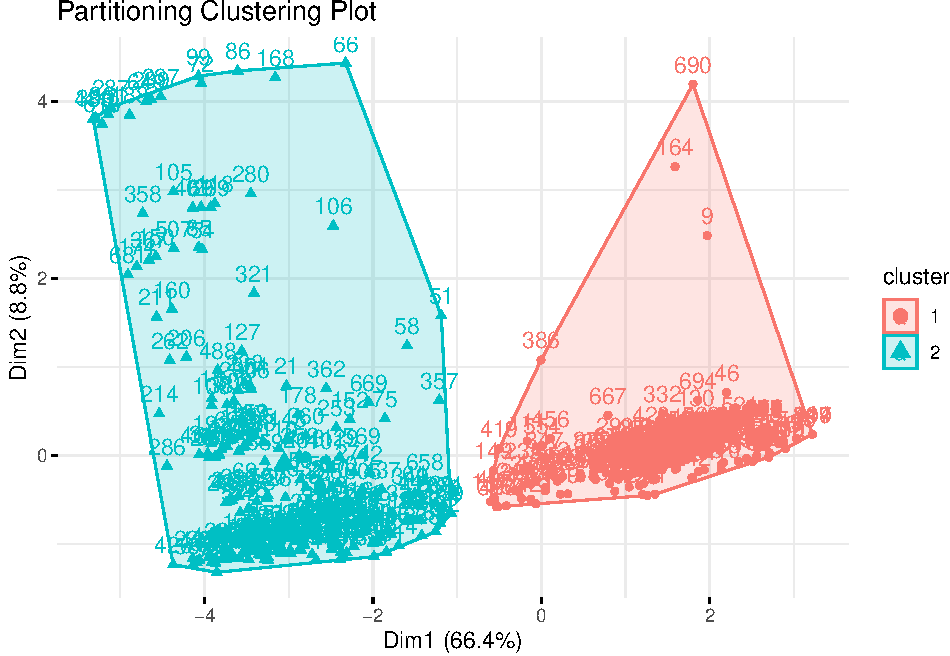
\includegraphics[width=0.7\linewidth]{Práctica-R-Clustering_files/figure-latex/unnamed-chunk-15-1} \end{center}

\begin{Shaded}
\begin{Highlighting}[]
\NormalTok{sil <-}\StringTok{ }\KeywordTok{silhouette}\NormalTok{(km_clusters}\OperatorTok{$}\NormalTok{cluster, }\KeywordTok{dist}\NormalTok{(BreastCancer.features))}
\KeywordTok{fviz_silhouette}\NormalTok{(sil)}
\end{Highlighting}
\end{Shaded}

\begin{verbatim}
##   cluster size ave.sil.width
## 1       1  435          0.59
## 2       2  248          0.44
\end{verbatim}

\begin{center}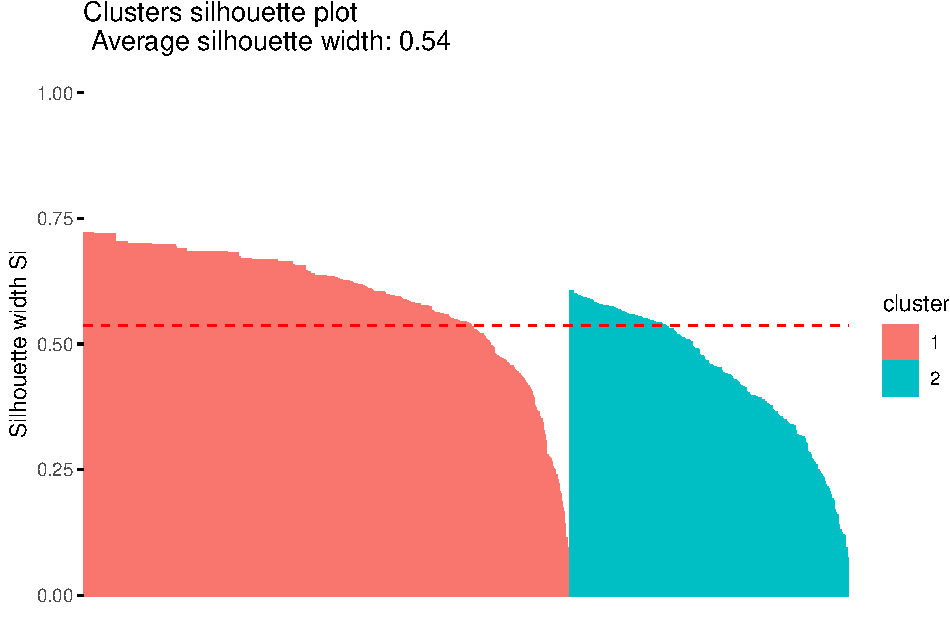
\includegraphics[width=0.7\linewidth]{Práctica-R-Clustering_files/figure-latex/unnamed-chunk-15-2} \end{center}

El resultado de agrupamiento sí presenta mejoras. Los clusters están más
definidos. Ya no existe \emph{overlapping} entre ellos.

\begin{itemize}
\tightlist
\item
  c(``range'')
\end{itemize}

\begin{Shaded}
\begin{Highlighting}[]
\CommentTok{#INSERTAR CÓDIGO AQUÍ}
\NormalTok{BreastCancer.scale <-}\StringTok{ }\KeywordTok{preProcess}\NormalTok{(BreastCancer[, }\DecValTok{1}\OperatorTok{:}\DecValTok{9}\NormalTok{], }\DataTypeTok{method=}\KeywordTok{c}\NormalTok{(}\StringTok{"range"}\NormalTok{))}
\NormalTok{BreastCancer.features <-}\StringTok{ }\KeywordTok{predict}\NormalTok{(BreastCancer.scale, BreastCancer[, }\DecValTok{1}\OperatorTok{:}\DecValTok{9}\NormalTok{])}
\KeywordTok{set.seed}\NormalTok{(}\DecValTok{101}\NormalTok{)}
\NormalTok{km_clusters <-}\StringTok{ }\KeywordTok{kmeans}\NormalTok{(BreastCancer.features, }\DataTypeTok{centers =} \DecValTok{2}\NormalTok{, }\DataTypeTok{nstart =} \DecValTok{20}\NormalTok{)}
\KeywordTok{fviz_cluster}\NormalTok{(km_clusters, }\DataTypeTok{data =}\NormalTok{ BreastCancer.features,}
             \DataTypeTok{ggtheme =} \KeywordTok{theme_minimal}\NormalTok{(),}
             \DataTypeTok{main =} \StringTok{"Partitioning Clustering Plot"}\NormalTok{)}
\end{Highlighting}
\end{Shaded}

\begin{center}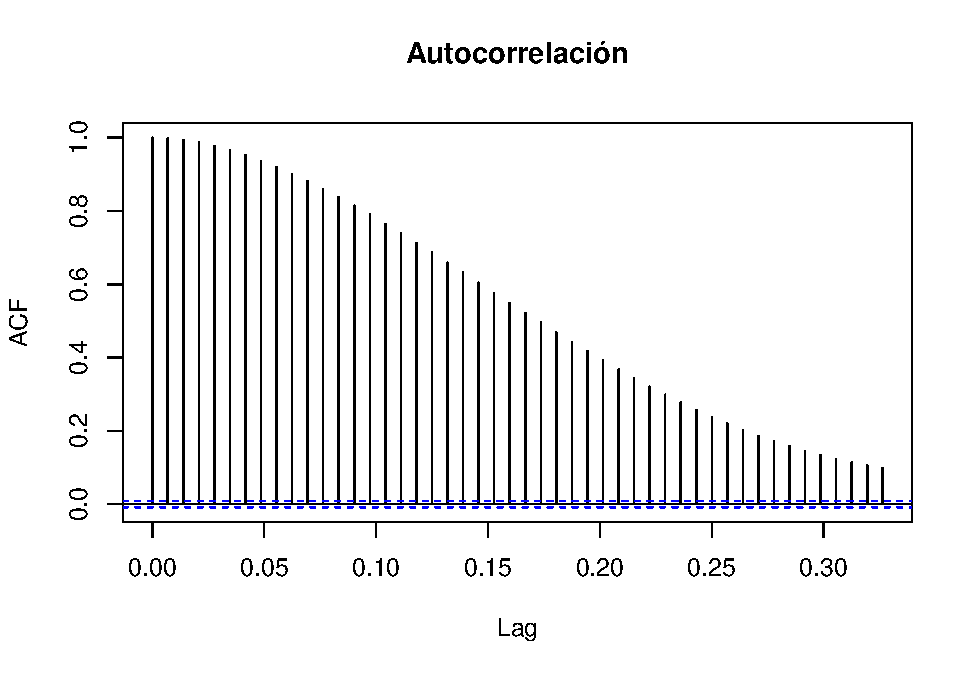
\includegraphics[width=0.7\linewidth]{Práctica-R-Clustering_files/figure-latex/unnamed-chunk-16-1} \end{center}

\begin{Shaded}
\begin{Highlighting}[]
\NormalTok{sil <-}\StringTok{ }\KeywordTok{silhouette}\NormalTok{(km_clusters}\OperatorTok{$}\NormalTok{cluster, }\KeywordTok{dist}\NormalTok{(BreastCancer.features))}
\KeywordTok{fviz_silhouette}\NormalTok{(sil)}
\end{Highlighting}
\end{Shaded}

\begin{verbatim}
##   cluster size ave.sil.width
## 1       1  453          0.76
## 2       2  230          0.28
\end{verbatim}

\begin{center}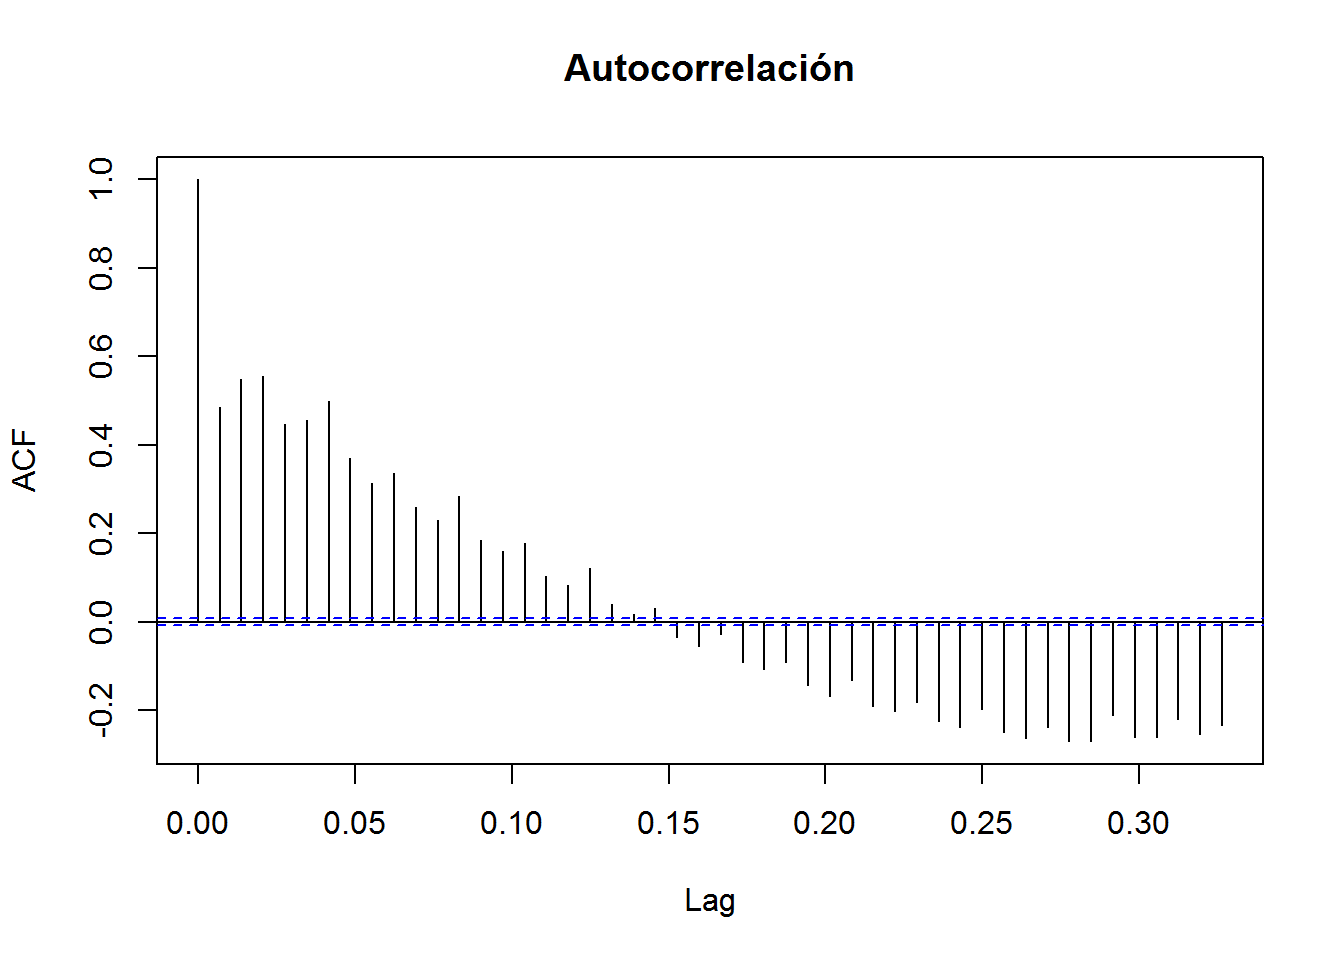
\includegraphics[width=0.7\linewidth]{Práctica-R-Clustering_files/figure-latex/unnamed-chunk-16-2} \end{center}

El resultado de agrupamiento sí presenta mejoras.

\begin{itemize}
\tightlist
\item
  c(``range'', ``YeoJohnson'')
\end{itemize}

\begin{Shaded}
\begin{Highlighting}[]
\CommentTok{#INSERTAR CÓDIGO AQUÍ}
\NormalTok{BreastCancer.scale <-}\StringTok{ }\KeywordTok{preProcess}\NormalTok{(BreastCancer[, }\DecValTok{1}\OperatorTok{:}\DecValTok{9}\NormalTok{], }\DataTypeTok{method=}\KeywordTok{c}\NormalTok{(}\StringTok{"range"}\NormalTok{, }\StringTok{"YeoJohnson"}\NormalTok{))}
\NormalTok{BreastCancer.features <-}\StringTok{ }\KeywordTok{predict}\NormalTok{(BreastCancer.scale, BreastCancer[, }\DecValTok{1}\OperatorTok{:}\DecValTok{9}\NormalTok{])}
\KeywordTok{set.seed}\NormalTok{(}\DecValTok{101}\NormalTok{)}
\NormalTok{km_clusters <-}\StringTok{ }\KeywordTok{kmeans}\NormalTok{(BreastCancer.features, }\DataTypeTok{centers =} \DecValTok{2}\NormalTok{, }\DataTypeTok{nstart =} \DecValTok{20}\NormalTok{)}
\KeywordTok{fviz_cluster}\NormalTok{(km_clusters, }\DataTypeTok{data =}\NormalTok{ BreastCancer.features,}
             \DataTypeTok{ggtheme =} \KeywordTok{theme_minimal}\NormalTok{(),}
             \DataTypeTok{main =} \StringTok{"Partitioning Clustering Plot"}\NormalTok{)}
\end{Highlighting}
\end{Shaded}

\begin{center}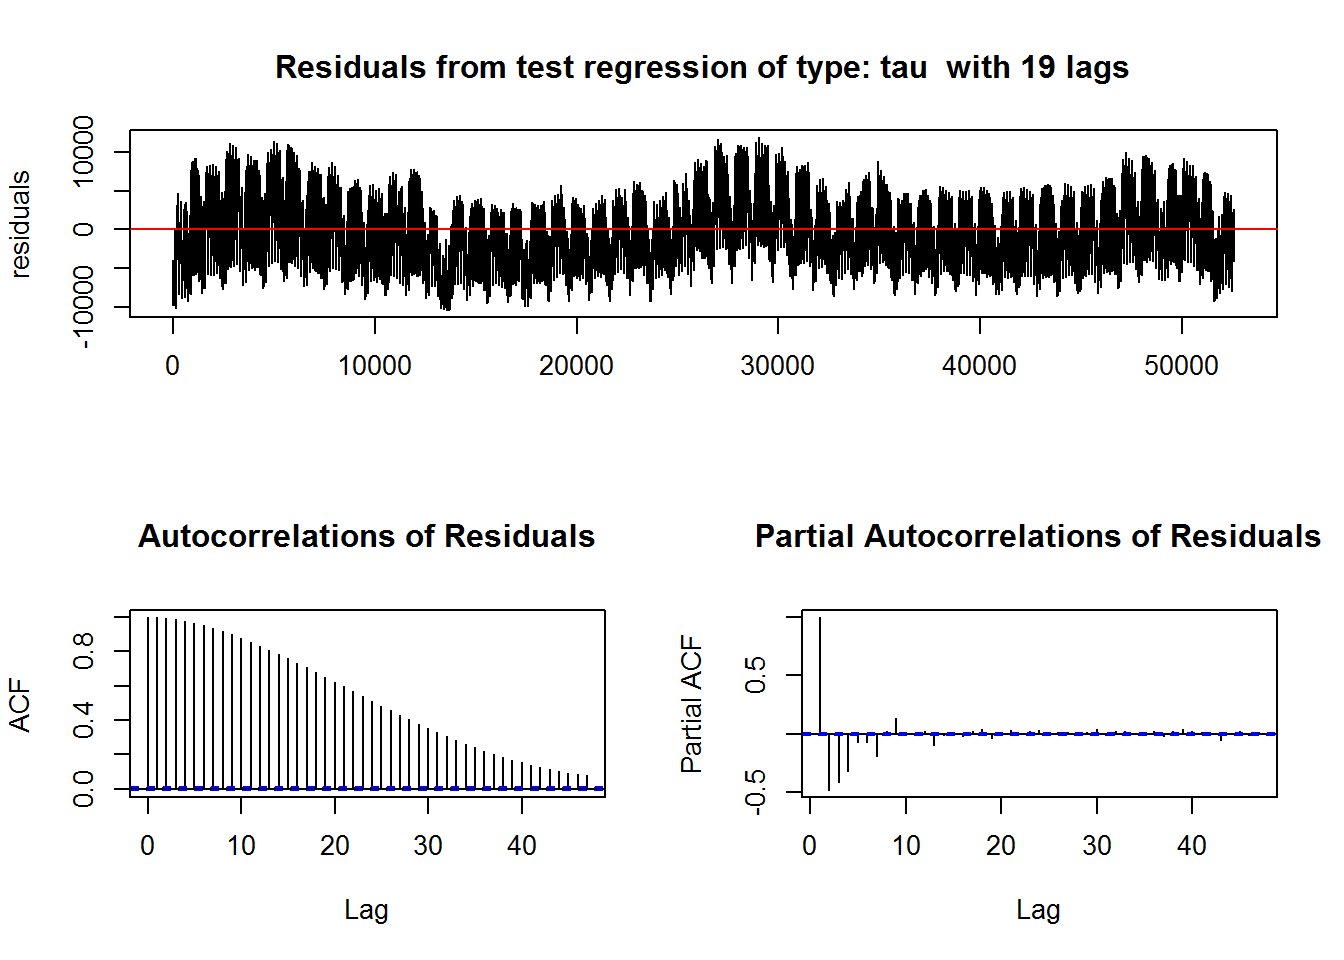
\includegraphics[width=0.7\linewidth]{Práctica-R-Clustering_files/figure-latex/unnamed-chunk-17-1} \end{center}

\begin{Shaded}
\begin{Highlighting}[]
\NormalTok{sil <-}\StringTok{ }\KeywordTok{silhouette}\NormalTok{(km_clusters}\OperatorTok{$}\NormalTok{cluster, }\KeywordTok{dist}\NormalTok{(BreastCancer.features))}
\KeywordTok{fviz_silhouette}\NormalTok{(sil)}
\end{Highlighting}
\end{Shaded}

\begin{verbatim}
##   cluster size ave.sil.width
## 1       1  433          0.61
## 2       2  250          0.50
\end{verbatim}

\begin{center}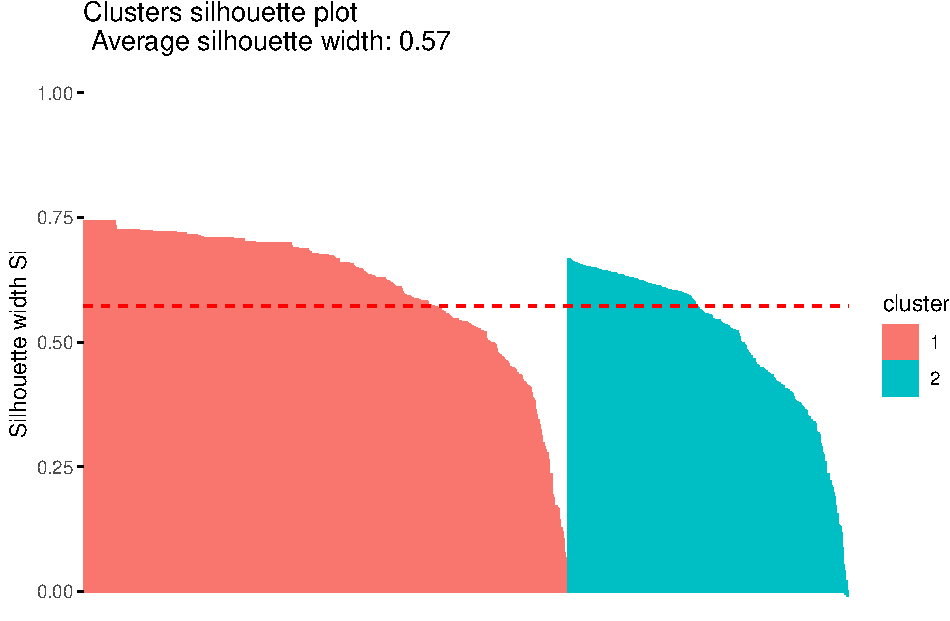
\includegraphics[width=0.7\linewidth]{Práctica-R-Clustering_files/figure-latex/unnamed-chunk-17-2} \end{center}

El resultado de agrupamiento no presenta mejoras.

\begin{itemize}
\tightlist
\item
  A partir del par de variables seleccionadas, cree un agrupamiento
  conformado por tres variables; las dos variables previamente
  seleccionadas y otra variable seleccionada aleatoriamente entre las
  variables descriptoras restantes. Este proceso debes repetirlo cinco
  veces de tal manera que en cada ejecución la variable añadida no
  necesariamente sea la misma.
\end{itemize}

\begin{Shaded}
\begin{Highlighting}[]
\CommentTok{#INSERTAR CÓDIGO AQUÍ}
\NormalTok{BreastCancer.scale <-}\StringTok{ }\KeywordTok{preProcess}\NormalTok{(BreastCancer[, }\DecValTok{1}\OperatorTok{:}\DecValTok{9}\NormalTok{], }\DataTypeTok{method=}\KeywordTok{c}\NormalTok{(}\StringTok{"scale"}\NormalTok{))}
\NormalTok{BreastCancer.features <-}\StringTok{ }\KeywordTok{predict}\NormalTok{(BreastCancer.scale, BreastCancer[, }\DecValTok{1}\OperatorTok{:}\DecValTok{9}\NormalTok{])}

\NormalTok{func <-}\StringTok{ }\ControlFlowTok{function}\NormalTok{ (var) \{ }
\NormalTok{  new_data <-}\StringTok{ }\KeywordTok{c}\NormalTok{(}\StringTok{"Cell.size"}\NormalTok{, }\StringTok{"Cell.shape"}\NormalTok{, var)}
  \KeywordTok{set.seed}\NormalTok{(}\DecValTok{101}\NormalTok{)}
\NormalTok{  km_clusters <-}\StringTok{ }\KeywordTok{kmeans}\NormalTok{(BreastCancer.features[new_data], }\DataTypeTok{centers =} \DecValTok{2}\NormalTok{, }\DataTypeTok{nstart =} \DecValTok{20}\NormalTok{)}
  \KeywordTok{fviz_cluster}\NormalTok{(km_clusters, }\DataTypeTok{data =}\NormalTok{ BreastCancer.features[, }\KeywordTok{c}\NormalTok{(}\StringTok{"Cell.size"}\NormalTok{, }\StringTok{"Cell.shape"}\NormalTok{)],}
             \DataTypeTok{ggtheme =} \KeywordTok{theme_minimal}\NormalTok{(),}
             \DataTypeTok{main =} \StringTok{"Partitioning Clustering Plot"}\NormalTok{)}
\NormalTok{\}}

\NormalTok{vars <-}\StringTok{ }\KeywordTok{c}\NormalTok{(}\StringTok{"Cl.thickness"}\NormalTok{, }\StringTok{"Marg.adhesion"}\NormalTok{, }\StringTok{"Epith.c.size"}\NormalTok{, }\StringTok{"Bare.nuclei"}\NormalTok{, }\StringTok{"Bl.cromatin"}\NormalTok{)}

\KeywordTok{func}\NormalTok{(vars[}\DecValTok{1}\NormalTok{])}
\end{Highlighting}
\end{Shaded}

\begin{center}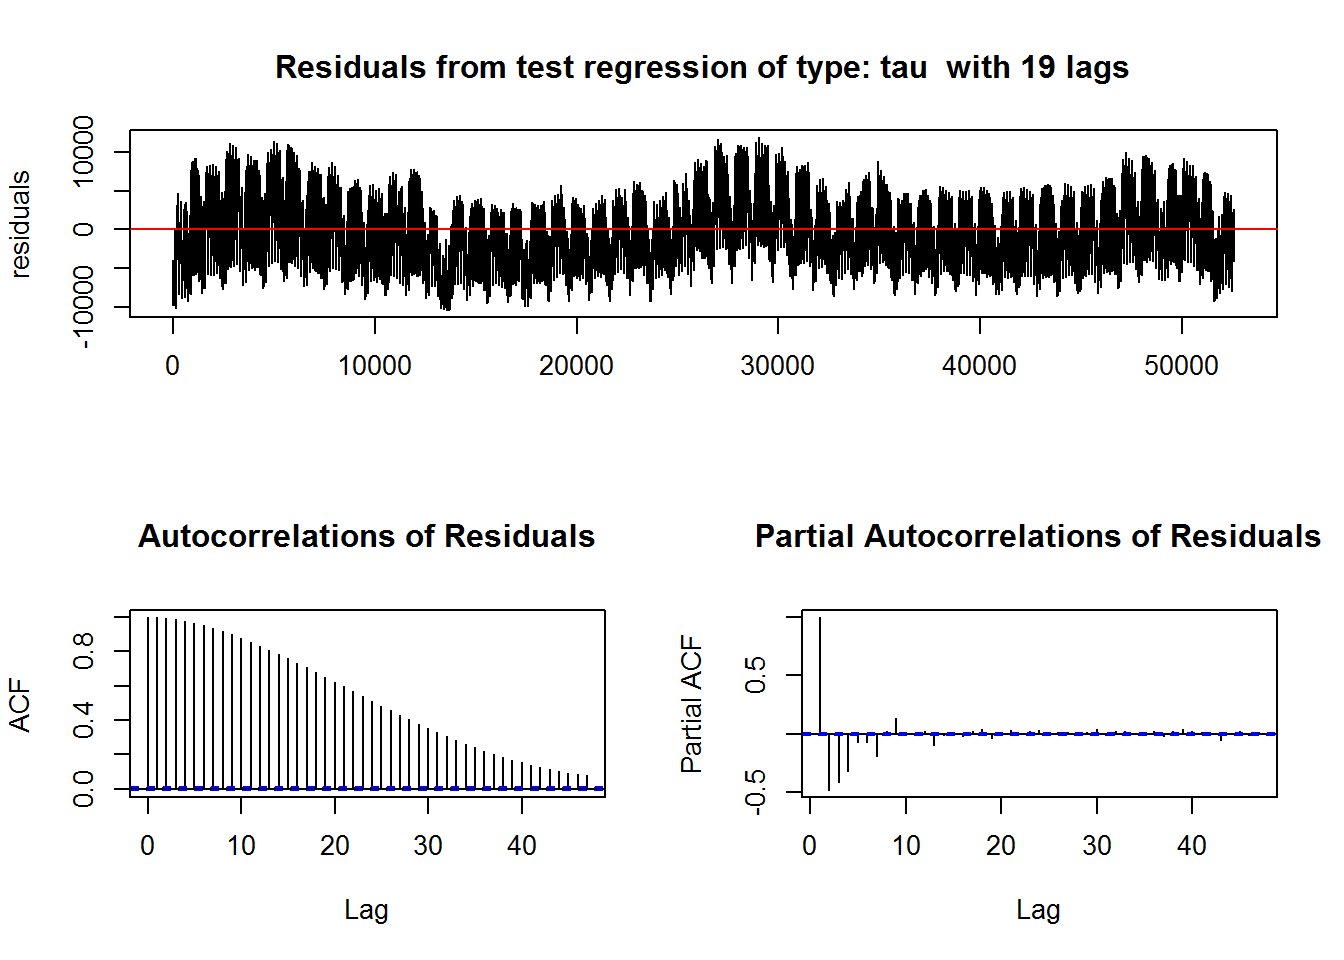
\includegraphics[width=0.7\linewidth]{Práctica-R-Clustering_files/figure-latex/unnamed-chunk-18-1} \end{center}

\begin{Shaded}
\begin{Highlighting}[]
\KeywordTok{func}\NormalTok{(vars[}\DecValTok{2}\NormalTok{])}
\end{Highlighting}
\end{Shaded}

\begin{center}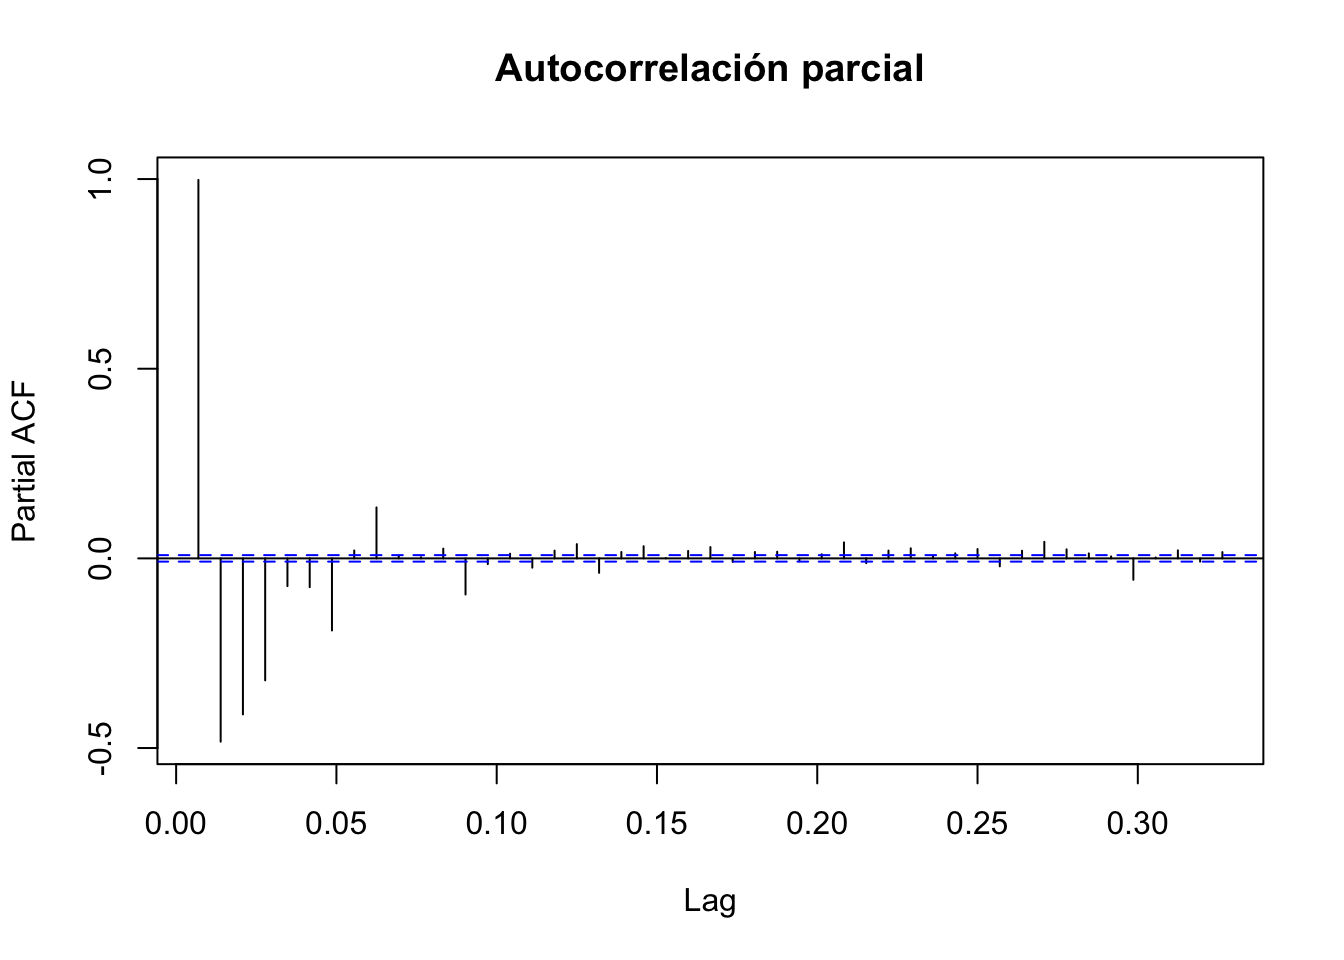
\includegraphics[width=0.7\linewidth]{Práctica-R-Clustering_files/figure-latex/unnamed-chunk-18-2} \end{center}

\begin{Shaded}
\begin{Highlighting}[]
\KeywordTok{func}\NormalTok{(vars[}\DecValTok{3}\NormalTok{])}
\end{Highlighting}
\end{Shaded}

\begin{center}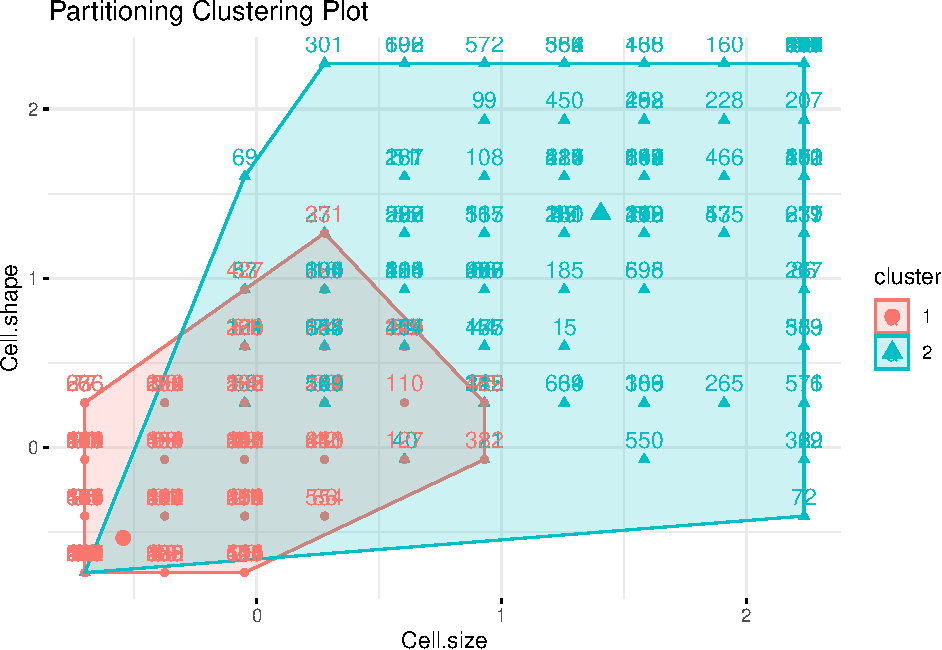
\includegraphics[width=0.7\linewidth]{Práctica-R-Clustering_files/figure-latex/unnamed-chunk-18-3} \end{center}

\begin{Shaded}
\begin{Highlighting}[]
\KeywordTok{func}\NormalTok{(vars[}\DecValTok{4}\NormalTok{])}
\end{Highlighting}
\end{Shaded}

\begin{center}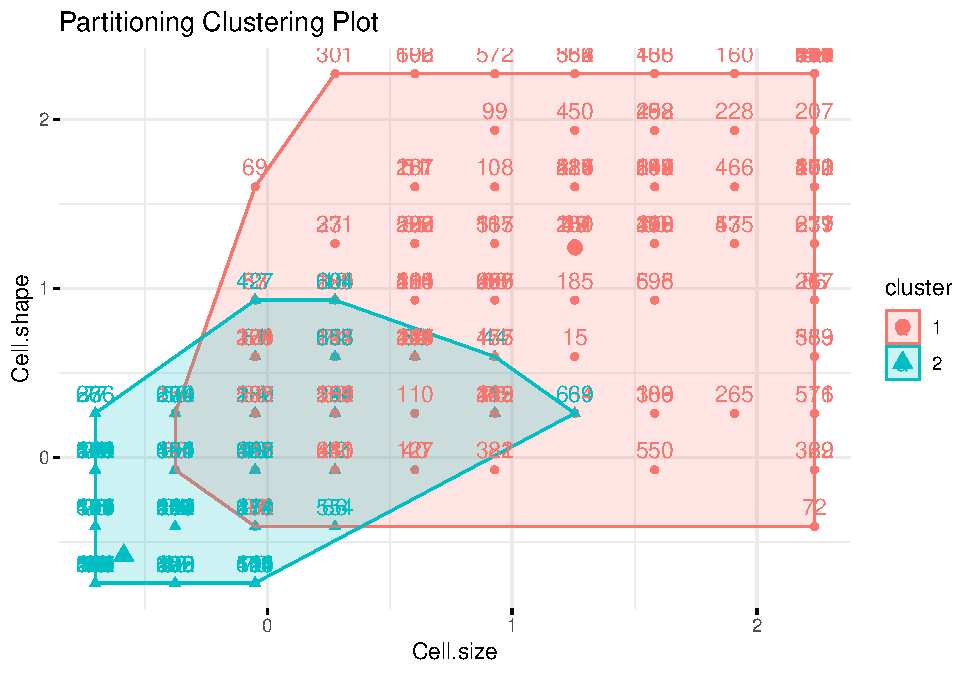
\includegraphics[width=0.7\linewidth]{Práctica-R-Clustering_files/figure-latex/unnamed-chunk-18-4} \end{center}

\begin{Shaded}
\begin{Highlighting}[]
\KeywordTok{func}\NormalTok{(vars[}\DecValTok{5}\NormalTok{])}
\end{Highlighting}
\end{Shaded}

\begin{center}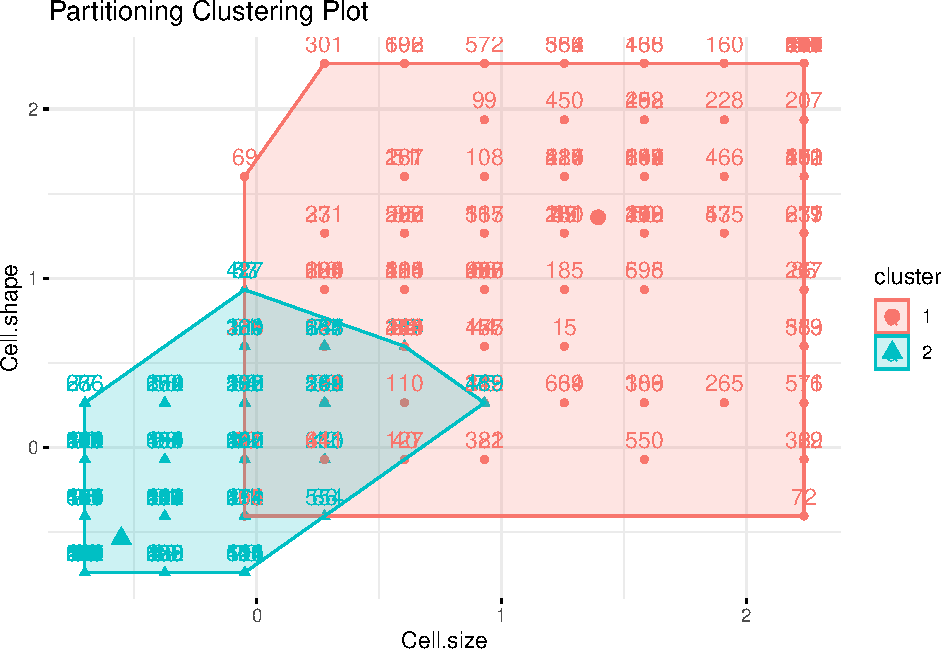
\includegraphics[width=0.7\linewidth]{Práctica-R-Clustering_files/figure-latex/unnamed-chunk-18-5} \end{center}

\begin{itemize}
\tightlist
\item
  A partir de los resultados obtenidos responda lo siguiente, ¿Tiene
  alguna ventaja o desventaja incluir más variables? ¿Qué posible
  explicación puedes darle a los resultados?
\end{itemize}

En todos los casos es una desventaja. Al incluir más variables los dos
clusters se agrupan incorrectamente. Vemos como existe
\emph{overlapping}.

\hypertarget{clustering-jeruxe1rquico}{%
\subsubsection{Clustering jerárquico}\label{clustering-jeruxe1rquico}}

Como hemos visto, con kmeans debemos de especificar a priori el número
de clusters que queremos obtener. Dado que el clustering es una tarea de
aprendizaje no supervisado, en algunos casos puede que no tengamos esa
información a priori, por lo que necesitaremos de otro tipo de técnicas,
como por ejemplo el agrupamiento jerárquico. Un agrupamiento jerárquico
en R se puede realizar mediante la función hclust(..), para ello debemos
especificar el tipo de método de aglomeración a usar.

\begin{itemize}
\tightlist
\item
  Crea un agrupamiento jerárquico usando hclust(..), para ello debe
  encontrar el método de aglomeración que mejor agrupa los tipos de
  cáncer. Una vez encontrado el mejor método, gráfica un dendograma que
  muestre información sobre el agrupamiento.
\end{itemize}

Nota: Consulta la ayuda de la función hclust(..) para ver los tipos de
métodos de aglomeración que soporta. También puedes ayudarte de las
funciones table(..) y plot(..) para realizar tu elección final. Además,
recuerda que no debes tener en cuenta la variable Class cuando ejecutas
la función hclust(..).

\begin{Shaded}
\begin{Highlighting}[]
\CommentTok{#INSERTAR CÓDIGO AQUÍ}
\NormalTok{dendrogram <-}\StringTok{ }\KeywordTok{hclust}\NormalTok{(}\KeywordTok{dist}\NormalTok{(BreastCancer.features, }\DataTypeTok{method =} \StringTok{'euclidean'}\NormalTok{), }\DataTypeTok{method =} \StringTok{'ward.D'}\NormalTok{)}
\KeywordTok{ggdendrogram}\NormalTok{(dendrogram, }\DataTypeTok{rotate =} \OtherTok{FALSE}\NormalTok{, }\DataTypeTok{labels =} \OtherTok{FALSE}\NormalTok{, }\DataTypeTok{theme_dendro =} \OtherTok{TRUE}\NormalTok{) }\OperatorTok{+}\StringTok{ }\KeywordTok{labs}\NormalTok{(}\DataTypeTok{title =} \StringTok{"Dendrograma"}\NormalTok{)}
\end{Highlighting}
\end{Shaded}

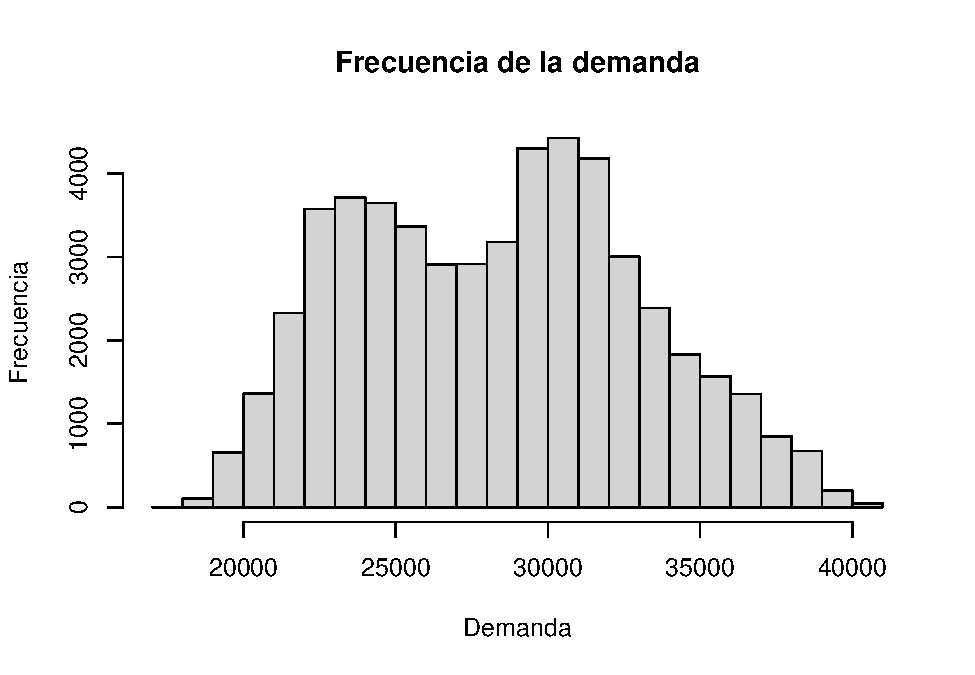
\includegraphics{Práctica-R-Clustering_files/figure-latex/unnamed-chunk-19-1.pdf}

\begin{itemize}
\tightlist
\item
  ¿Por qué el dendograma tendrá tantos grupos en el nivel más bajo?
  ¿Coincide este número con algún otro? Justifica.
\end{itemize}

RESPUESTA:

\begin{itemize}
\tightlist
\item
  ¿Por qué es necesario usar la función dist(..) al llamar a hclust(..)
  ?
\end{itemize}

RESPUESTA:

\begin{itemize}
\tightlist
\item
  ¿Por qué no es necesario usar set.seed(..) antes de llamar a
  hclust(..) ?
\end{itemize}

RESPUESTA:

\begin{itemize}
\tightlist
\item
  Debido a que hclust puede crear un número elevado de clústers, utilice
  la función cutree(..) para fijar el número de clúster igual al número
  de clases existentes en el dataset.
\end{itemize}

\begin{Shaded}
\begin{Highlighting}[]
\CommentTok{#INSERTAR CÓDIGO AQUÍ}
\NormalTok{agrupamientoJ <-}\StringTok{ }\KeywordTok{hclust}\NormalTok{(}\KeywordTok{dist}\NormalTok{(BreastCancer.features, }\DataTypeTok{method =} \StringTok{'euclidean'}\NormalTok{), }\DataTypeTok{method =} \StringTok{'ward.D'}\NormalTok{)}
\NormalTok{clases_aj <-}\StringTok{ }\KeywordTok{cutree}\NormalTok{(agrupamientoJ, }\DataTypeTok{k =} \DecValTok{2}\NormalTok{)}
\NormalTok{BreastCancer.features}\OperatorTok{$}\NormalTok{cluster <-}\StringTok{ }\NormalTok{clases_aj}
\NormalTok{clusters <-}\StringTok{ }\NormalTok{BreastCancer.features}\OperatorTok{$}\NormalTok{cluster}

\KeywordTok{ggplot}\NormalTok{(BreastCancer, }\KeywordTok{aes}\NormalTok{(Cell.size, Cell.shape, }\DataTypeTok{color =} \KeywordTok{as.factor}\NormalTok{(clusters))) }\OperatorTok{+}\StringTok{ }\KeywordTok{geom_point}\NormalTok{()}
\end{Highlighting}
\end{Shaded}

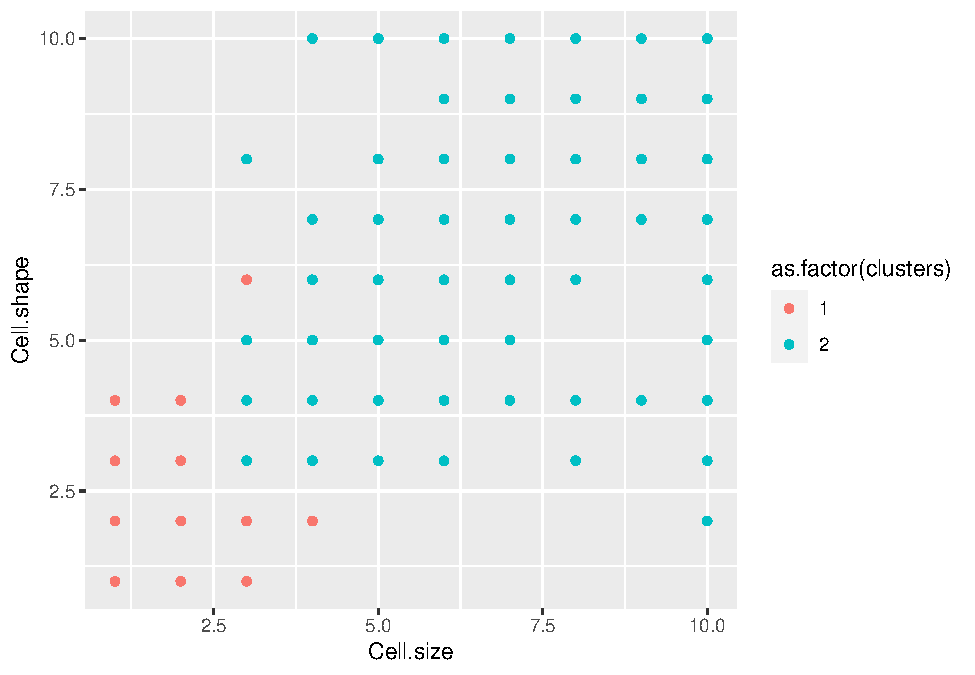
\includegraphics{Práctica-R-Clustering_files/figure-latex/unnamed-chunk-20-1.pdf}

\begin{Shaded}
\begin{Highlighting}[]
\KeywordTok{table}\NormalTok{(BreastCancer}\OperatorTok{$}\NormalTok{Class, clusters)}
\end{Highlighting}
\end{Shaded}

\begin{verbatim}
##            clusters
##               1   2
##   benign    412  32
##   malignant   2 237
\end{verbatim}

-¿Cuando hacemos esta última operación con la función cutree(..), el
agrupamiento que obtenemos por hclust(..) es mejor al obtenido con
kMeans en el ejercicio anterior?

RESPUESTA:

\end{document}
